\documentclass[border=10pt]{standalone}

\usepackage{tikz}
\usepackage{tikzsymbols}
\usetikzlibrary{calc,patterns,shapes.geometric}

\def\centerarc[#1](#2)(#3:#4:#5){\draw[#1] ($(#2)+({#5*cos(#3)},{#5*sin(#3)})$) arc (#3:#4:#5);}

\begin{document}
	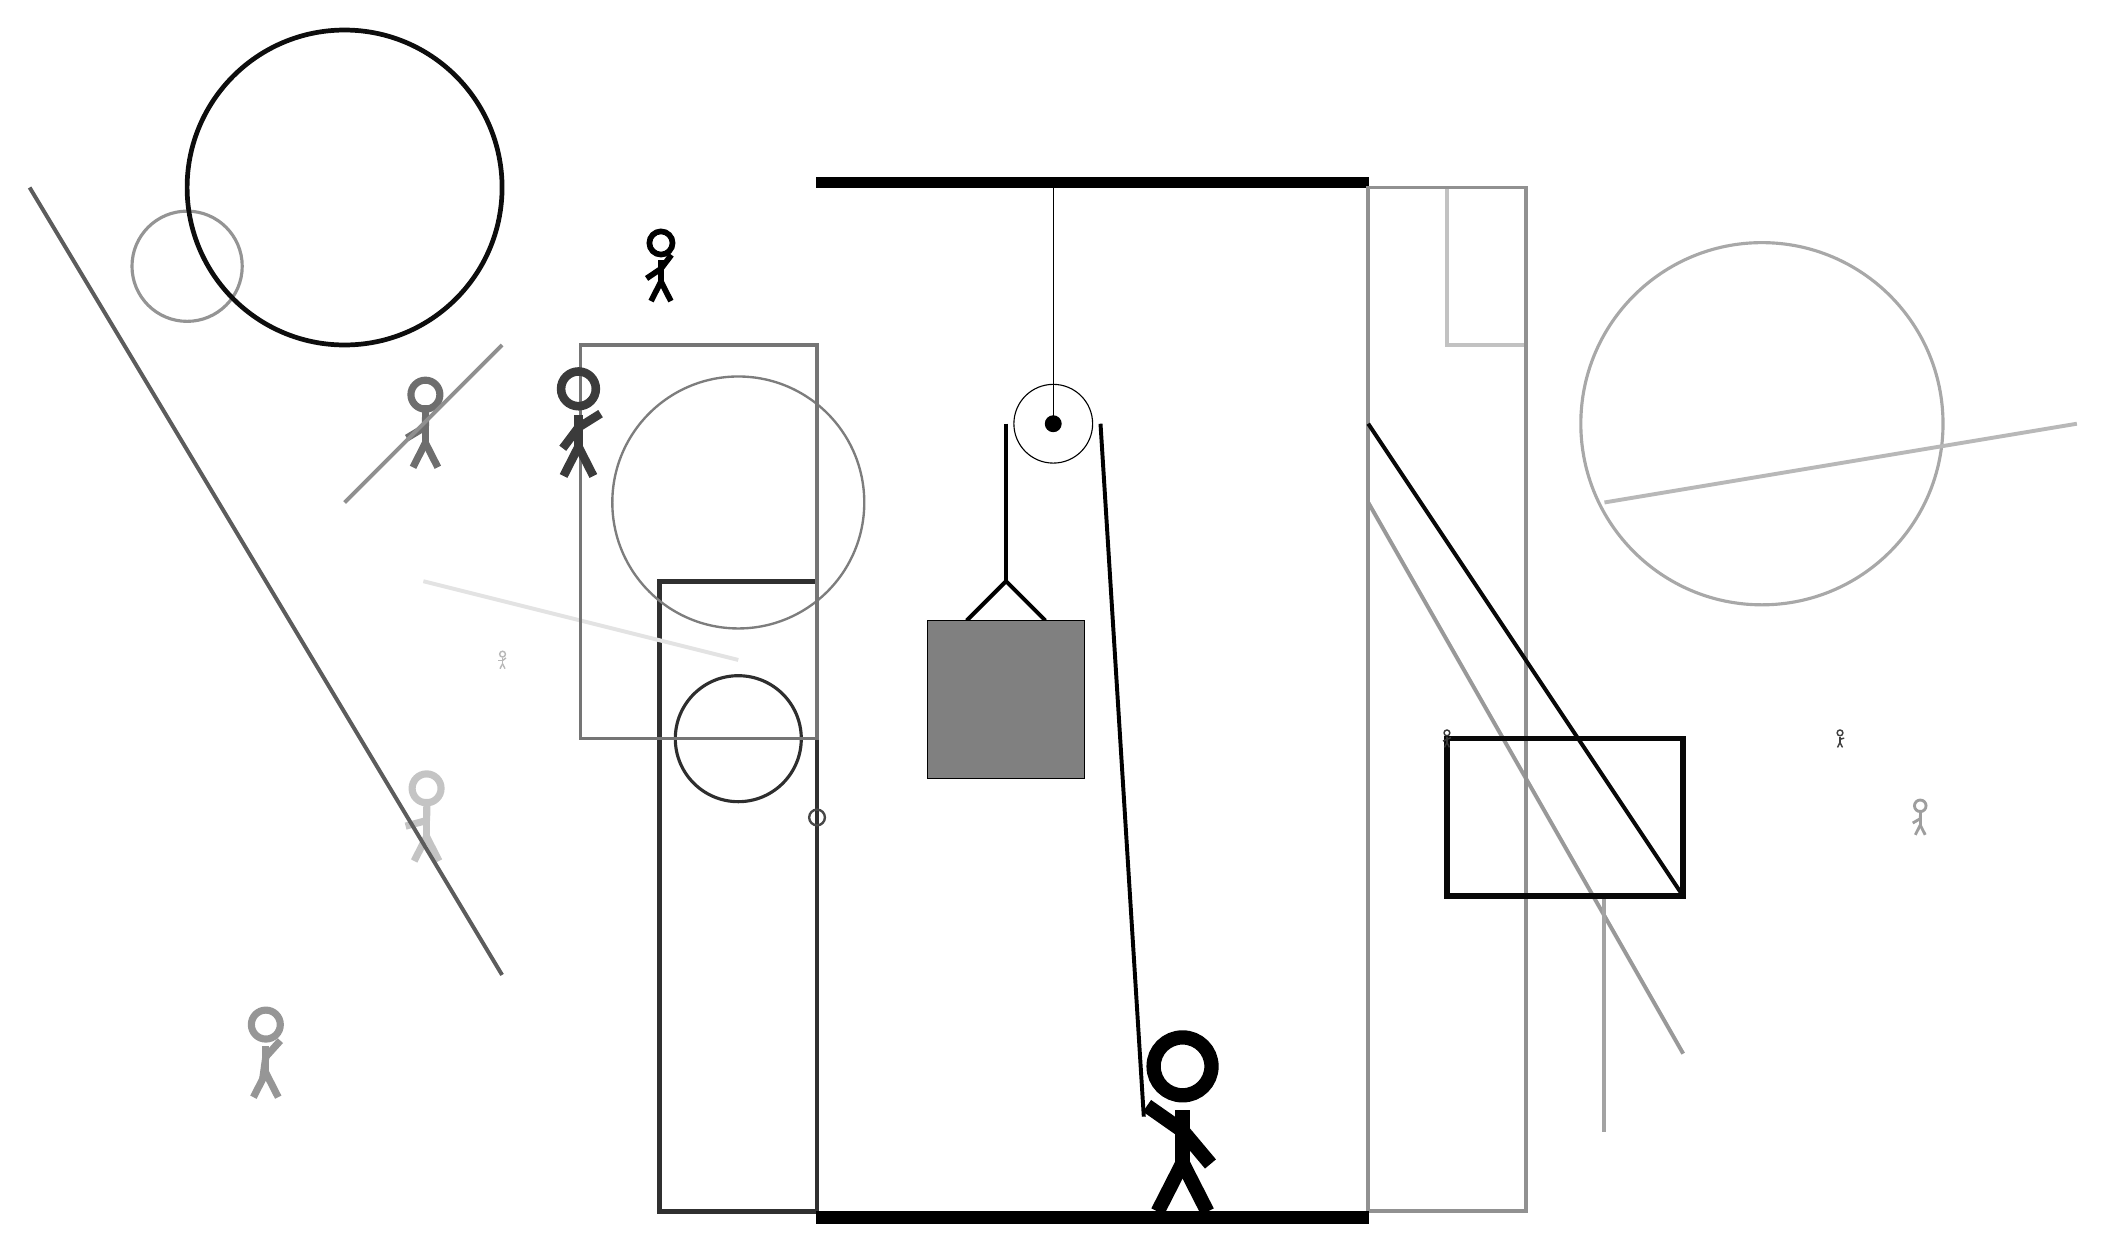
\begin{tikzpicture}
		%%%%% START %%%%%
		
		\draw[fill=black] (-2, 10) rectangle (5, 10.125);
		
		\draw (1, 7) circle (0.5);
		\draw[fill=black] (1, 7) circle (0.1);
		\draw (1, 10) -- (1, 7);
		
		\draw [line width=0.4mm, color=black!34](10, 7) circle (2.3);
		
		\draw[line width=0.6mm, color=black!81] (-2, 5) rectangle (-4, -3);
		\draw[line width=0.5mm, color=black!93](-4, 5) -- (-4, 5);
		\node[line width=0.7mm, color=black!23] at (-7, 2) {\Strichmaxerl[5][15][89]};
		\draw [line width=0.3mm, color=black!51](-3, 6) circle (1.6);
		\node[line width=0.7mm, color=black!57] at (-7, 7) {\Strichmaxerl[5][31][89]};
		
		\draw [line width=0.3mm, color=black!72](-2, 2) circle (0.1);
		
		\draw[line width=0.5mm, color=black!40](9, -1) -- (5, 6);
		\draw[line width=0.4mm, color=black!24] (7, 10) rectangle (6, 8);
		\draw [line width=0.4mm, color=black!82](-3, 3) circle (0.8);
		\draw[line width=0.5mm, color=black!28](8, 6) -- (14, 7);
		
		\draw [line width=0.2mm, color=black!25](-9, -2) circle (0.0);
		\draw[line width=0.5mm, color=black!44](-6, 8) -- (-8, 6);
		
		\node[line width=0.7mm, color=black!38] at (12, 2) {\Strichmaxerl[2][30][87]};
		\draw[line width=0.5mm, color=black!43] (5, 10) rectangle (7, -3);
		\node[line width=0.7mm, color=black!28] at (-6, 4) {\Strichmaxerl[1][0][38]};
		
		\draw[line width=0.5mm, color=black!11](-7, 5) -- (-3, 4);
		
		\draw[line width=0.5mm, color=black!97](9, 1) -- (5, 7);
		\draw [line width=0.4mm, color=black!42](-10, 9) circle (0.7);
		
		\node[line width=0.2mm, color=black!75] at (11, 3) {\Strichmaxerl[1][85][16]};
		\draw[line width=0.4mm, color=black!54] (-2, 8) rectangle (-5, 3);
		
		\node[line width=0.4mm, color=black!77] at (-5, 7) {\Strichmaxerl[6][53][32]};
		\node[line width=0.7mm, color=black!41] at (-9, -1) {\Strichmaxerl[5][82][48]};
		\draw [line width=0.6mm, color=black!95](-8, 10) circle (2.0);
		\node[line width=0.7mm, color=black!100] at (-4, 9) {\Strichmaxerl[4][34][53]};
		\draw[line width=0.5mm, color=black!64](-6, 0) -- (-12, 10);
		\draw[line width=0.5mm, color=black!36](8, 1) -- (8, -2);
		\draw[line width=0.7mm, color=black!97] (6, 1) rectangle (9, 3);
		\node[line width=0.6mm, color=black!78] at (6, 3) {\Strichmaxerl[1][24][23]};
		
		\draw[line width=0.5mm] (-0.1, 4.5) -- (0.4, 5.0) -- (0.9, 4.5);
		\draw[fill=black!50] (-0.6, 4.5) rectangle (1.4, 2.5);
		
		\draw[line width=0.5mm] (0.4, 7) -- (0.4, 5.0);
		\centerarc[line width=0.5mm](1, 7)(0:180:0.6);
		\draw[line width=0.5mm](1.6, 7) -- (2.15, -1.8);
		
		\node at (2.6, -1.9) {\Strichmaxerl[10][-35][-50]};
		
		\draw[fill=black] (-2, -3) rectangle (5, -3.15);
		
		%%%%% END %%%%%
	\end{tikzpicture}
\end{document}